
\begin{figure}
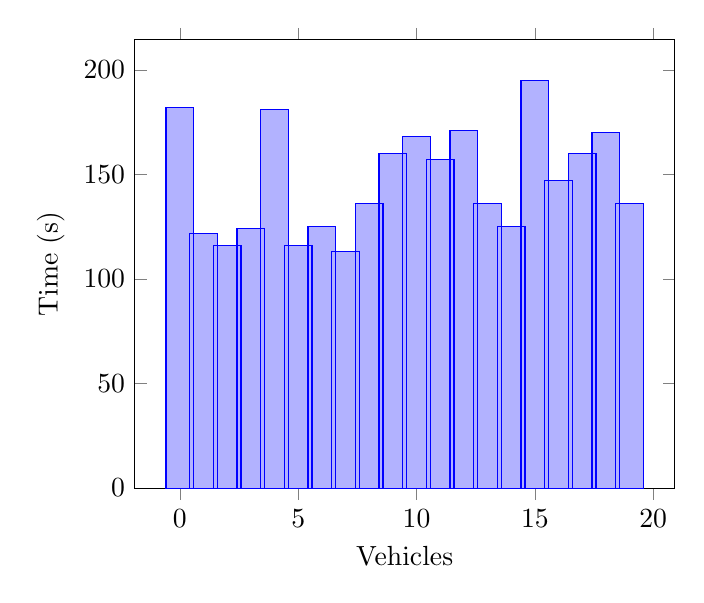
\begin{tikzpicture}
\begin{axis}[
legend style={anchor=west},
xlabel=Vehicles,
ylabel=Time (s),
ymin=0,
ybar,
]
\addplot coordinates {
(0, 182)
(1, 122)
(2, 116)
(3, 124)
(4, 181)
(5, 116)
(6, 125)
(7, 113)
(8, 136)
(9, 160)
(10, 168)
(11, 157)
(12, 171)
(13, 136)
(14, 125)
(15, 195)
(16, 147)
(17, 160)
(18, 170)
(19, 136)
};

\end{axis}
\end{tikzpicture}
\label{tik:100:18_N, 18_N.-60, 17_N, 15_S, 15_S.-30, 13_N, 13_N.-40, 11_N, 8_N, 7_N, 7_N.-60, 5_N, 4_N, 4_N.-60, 3_O}
\caption{100 percent diving with GSC on route $18_N, 18_N.-60, 17_N, 15_S, 15_S.-30, 13_N, 13_N.-40, 11_N, 8_N, 7_N, 7_N.-60, 5_N, 4_N, 4_N.-60, 3_O$}
\end{figure}
